\documentclass{article}

\usepackage[utf8]{inputenc}
\usepackage[T1]{fontenc}
\usepackage[french]{babel}
\usepackage{graphicx}
\usepackage{svg}
\usepackage{url}
\usepackage{float}
\usepackage{listings}
\usepackage{xcolor}
\definecolor{backgray}{rgb}{0.95,0.95,0.96}
\definecolor{cGreen}{rgb}{0,0.6,0}
\definecolor{cBlue}{rgb}{0,0,0.8}
\definecolor{cRed}{rgb}{0.6,0,0}
\definecolor{cGray}{rgb}{0.5,0.5,0.5}
\lstdefinestyle{styleCStandard}{
    language=C,
    backgroundcolor=\color{backgray},
    commentstyle=\color{cGreen},
    keywordstyle=\color{cBlue}\bfseries,
    stringstyle=\color{cRed},
    basicstyle=\ttfamily\footnotesize,
    numbers=left,
    numberstyle=\tiny\color{cGray},
    numbersep=5pt,
    frame=lines,
    breaklines=true,
    captionpos=t,
    tabsize=4,
    showspaces=false,
    showstringspaces=false,
    literate=
        {é}{{\'e}}1
        {è}{{\`e}}1
        {à}{{\`a}}1
        {ç}{{\c{c}}}1
        {ù}{{\`u}}1
        {ê}{{\^e}}1
        {î}{{\^i}}1
        {ô}{{\^o}}1
        {û}{{\^u}}1
        {ë}{{\"e}}1
        {ï}{{\"i}}1
        {'}{{'}}1
}
\lstset{style=styleCStandard}
\renewcommand{\lstlistingname}{Listing}
\usepackage[
  left=2cm,
  right=2cm,
  top=2.5cm,
  bottom=2.5cm
]{geometry}
\usepackage{amsmath}
\usepackage[colorlinks=true, allcolors=blue]{hyperref}


\usepackage[utf8]{inputenc}
\usepackage[T1]{fontenc}
\usepackage[french]{babel}
\usepackage{graphicx}
\usepackage{svg}
\usepackage{url}
\usepackage{float}
\usepackage[
  left=2cm,
  right=2cm,
  top=2.5cm,
  bottom=2.5cm
]{geometry}
\usepackage{amsmath}
\usepackage[colorlinks=true, allcolors=blue]{hyperref}

\title{PI\_ITInéraire\_26\_28}
\author{El Assad Ilyass / Kamara Mohamed / Ravier Mathis / Semy Julie / Thomas Ismaël}

\begin{document}
\maketitle
\tableofcontents

\newpage
\section{Analyse des capteurs disponibles}

\subsection{Choix des capteurs pour la fusion}
Le système d'acquisition de l'ITIPhone intègre quatre capteurs : un module GNSS
(DFRobot TEL0157), une centrale inertielle (MiniIMU-9 v6), un LiDAR 2D
(RPLIDAR A1M8) et une caméra (Raspberry Pi Camera Module 3). Cette section
justifie le choix des capteurs retenus pour la fusion de données.

\subsubsection{Module GNSS}

Le module GNSS fournit une position absolue en latitude et longitude à une
fréquence comprise entre 1 et 10~Hz. Son erreur est de nature
\textbf{stochastique et bornée} : les mesures oscillent aléatoirement autour
de la vraie position, sans dérive temporelle. Ce comportement est modélisé
par un bruit blanc gaussien de variance $\sigma^2_{\text{GPS}}$, typiquement de
l'ordre de quelques mètres carrés en milieu urbain.

Cependant, le GPS seul présente deux limitations majeures pour une estimation
de trajectoire robuste :

\begin{itemize}
    \item \textbf{Fréquence d'acquisition faible} : une mesure toutes les
    100~ms à 1~s est insuffisante pour restituer fidèlement une trajectoire
    lors d'un déplacement dynamique. Entre deux mesures, la position est
    inconnue.
    \item \textbf{Disponibilité conditionnelle} : en environnement urbain
    dense ou sous couvert végétal, le signal peut être temporairement
    indisponible, rendant l'estimation impossible sans capteur de substitution.
\end{itemize}

\subsubsection{Centrale inertielle IMU}

L'IMU MiniIMU-9 v6 intègre un accéléromètre, un gyroscope et un magnétomètre,
opérant à une fréquence typique de 100~Hz. La position est estimée par double
intégration numérique de l'accélération mesurée dans le repère monde :

\begin{align}
    \mathbf{v}(t) &= \mathbf{v}(t-1) + \mathbf{a}_{\text{monde}}(t) \cdot \Delta t \\
    \mathbf{x}(t) &= \mathbf{x}(t-1) + \mathbf{v}(t) \cdot \Delta t
\end{align}

L'IMU présente une limitation fondamentale : son erreur est \textbf{non
bornée}. Le biais $b$ de l'accéléromètre, après double intégration, produit
une erreur de position croissant en $t^2$ :

\begin{equation}
    \epsilon_{\text{position}}(t) \approx \frac{1}{2} \cdot b \cdot t^2
\end{equation}

Pour un biais typique de $b = 0{,}01$~m/s², l'erreur atteint 18~mètres après
60 secondes. \textbf{L'IMU seul est donc inutilisable pour une navigation de
longue durée.}

\subsubsection{LiDAR 2D et caméra}

Ces deux capteurs peuvent théoriquement fournir une estimation de déplacement
relatif (via l'algorithme ICP pour le LiDAR, ou l'odométrie visuelle pour la
caméra). Ils ont été écartés pour la fusion pour trois raisons :

\begin{itemize}
    \item Ils ne fournissent qu'un \textbf{déplacement relatif}, sans
    référence de position absolue — fonctionnellement équivalent à l'IMU,
    mais bien plus complexe à implémenter.
    \item Leurs performances en extérieur sont dégradées : l'ICP diverge dans
    les environnements peu structurés, et l'odométrie visuelle est sensible
     aux conditions lumineuses.
    \item Ces algorithmes sont coûteux en calcul pour une Raspberry Pi 4
    embarquée.
\end{itemize}

Ces capteurs seront valorisés dans le cadre de la Partie~2.

\subsection{Complémentarité GPS + IMU}

Le critère fondamental pour sélectionner les capteurs d'une fusion est la
\textbf{complémentarité de leurs caractéristiques d'erreur}. Le tableau
suivant résume les propriétés de chaque capteur :

\begin{table}[htbp]
    \centering
    \caption{Comparaison des caractéristiques d'erreur du GPS et de l'IMU}
    \begin{tabular}{lcc}
        \hline
        \textbf{Caractéristique} & \textbf{GPS} & \textbf{IMU} \\
        \hline
        Type d'erreur        & Bruit gaussien borné & Dérive en $t^2$ \\
        Fréquence            & 1--10~Hz             & $\sim$100~Hz    \\
        Fiabilité long terme & Bonne                & Mauvaise        \\
        Fiabilité court terme & Mauvaise (bruit)    & Bonne           \\
        Disponibilité        & Conditionnelle       & Permanente      \\
        \hline
    \end{tabular}
    \label{tab:capteurs}
\end{table}

La combinaison GPS + IMU est complémentaire sur chacun des problèmes identifiés :

\begin{enumerate}
    \item \textbf{Fréquence basse du GPS} : l'IMU à 100~Hz interpole la
    trajectoire entre deux mesures GPS, produisant un tracé continu et
    physiquement cohérent.
    \item \textbf{Perte de signal GPS} : l'IMU prend le relais en navigation
    autonome. Le filtre de Kalman modélise la dégradation progressive de
    la confiance via la matrice de covariance $\mathbf{P}$.
    \item \textbf{Bruit du GPS} : le filtre de Kalman combine les deux
    sources de manière optimale. On peut montrer que la variance de
    l'estimation fusionnée vérifie : la fusion de deux capteurs bruités produit
    donc \textbf{toujours une estimation plus précise} que le meilleur capteur
    pris seul, à condition que leurs bruits soient décorrélés — ce qui est
    vérifié ici, les deux capteurs reposant sur des principes physiques distincts.
\end{enumerate}


\section{Estimation de la trajectoire}

\subsection{Paramètres d'acquisition}
\label{sec:params}
Le module GNSS DFRobot TEL0157 offre plusieurs paramètres configurables,
notamment le choix de la constellation satellitaire et la fréquence
d'acquisition. Ces paramètres influencent directement la qualité des mesures
utilisées dans le filtre de Kalman. Une démarche expérimentale rigoureuse a
été menée pour déterminer la configuration optimale.

\subsection{Choix de la constellation GNSS}

\subsubsection{Problématique}

Le module TEL0157 supporte trois constellations satellitaires : GPS (américain),
BeiDou (chinois) et GLONASS (russe). Le système européen Galileo n'est pas
supporté par ce module il s'agit d'une limitation matérielle, non logicielle.
La question est la suivante : quelle combinaison de constellations offre le
meilleur compromis entre précision et robustesse pour notre application ?

\subsubsection{Protocole expérimental}

Trois acquisitions statiques ont été réalisées en extérieur, dans les mêmes
conditions, avec successivement chacune des trois configurations disponibles.
Le récepteur était posé immobile sur une surface plane dégagée, à l'abri de
tout obstacle susceptible de provoquer des réflexions multipath. Pour chaque
configuration, les coordonnées GPS ont été enregistrées sur plusieurs minutes,
puis analysées statistiquement.

Les indicateurs retenus sont :
\begin{itemize}
    \item $\sigma_{\text{lat}}$ et $\sigma_{\text{lon}}$ : écarts-types des
    mesures de latitude et longitude (en mètres), qui quantifient la dispersion
    autour de la position vraie.
    \item $\text{cov}(\text{lat}, \text{lon})$ : covariance croisée entre les
    deux axes, qui indique si les erreurs sont corrélées entre elles.
\end{itemize}

\subsubsection{Résultats}

\begin{table}[htbp]
    \centering
    \caption{Comparaison statistique des trois configurations de constellation
    (acquisition statique extérieure)}
    \begin{tabular}{lcccl}
        \hline
        \textbf{Configuration} & $\sigma_{\text{lat}}$ (m) &
        $\sigma_{\text{lon}}$ (m) & $\text{cov}$ (m²) &
        \textbf{Bruit gaussien ?} \\
        \hline
        GPS + BeiDou          & 4.15  & 8.71  & 19.64  & Non \\
        GPS seul              & 0.089 & 0.059 & $-$0.002 & Oui \\
        GPS + BeiDou + GLONASS & 0.262 & 1.095 & 0.006 & Oui \\
        \hline
    \end{tabular}
    \label{tab:constellations}
\end{table}

\subsubsection{Analyse et décision}

La configuration GPS + BeiDou est immédiatement écartée : sa covariance
croisée de 19.64~m² trahit une forte corrélation entre les erreurs de latitude
et de longitude. Ce comportement est incompatible avec l'hypothèse gaussienne
du filtre de Kalman, qui suppose des bruits décorrélés.

Les deux configurations restantes présentent toutes deux un bruit
quasi-gaussien décorrélé. Le GPS seul affiche un écart-type plus faible, mais
repose sur un nombre limité de satellites. En environnement partiellement
masqué (végétation, bâtiments), la disponibilité des satellites GPS seuls peut
se dégrader significativement, entraînant des pertes de signal et des sauts de
position importants. La configuration GPS + BeiDou + GLONASS exploite trois
constellations distinctes, augmentant le nombre de satellites visibles et
réduisant ainsi la probabilité de perte de signal.

\textbf{Décision retenue : GPS + BeiDou + GLONASS.} La légère dégradation
de la précision en conditions statiques idéales est compensée par une
meilleure robustesse en conditions réelles de marche, et reste tout à fait
gérable par le filtre de Kalman via la matrice de bruit de mesure $R$.

\subsubsection{Dérivation de la matrice de bruit de mesure $R$}

La covariance croisée quasi nulle ($\text{cov} = 0.006$~m²) confirme que les
erreurs sur les axes Est et Nord sont décorrélées. La matrice $R$ peut donc
être modélisée comme une matrice diagonale, dont les termes sont directement
issus des variances mesurées :

\begin{align}
    \sigma_{\text{lon}}^2 &= 1.095^2 \approx 1.20 \ \text{m}^2 \\
    \sigma_{\text{lat}}^2 &= 0.262^2 \approx 0.07 \ \text{m}^2
\end{align}

Ce qui donne :

\begin{equation}
    R = \begin{bmatrix} 1.20 & 0 \\ 0 & 0.07 \end{bmatrix} \quad \text{(m}^2\text{)}
\end{equation}

Cette matrice est utilisée telle quelle dans l'étape de correction du filtre
de Kalman Étendu, décrite en section~\ref{sec:ekf}.

\subsection{Fréquences d'acquisition}

\subsubsection{Module GNSS : 1~Hz}

Le module TEL0157 est configuré pour délivrer une trame de position à une fréquence de 1~Hz, soit une mesure toutes les secondes. Bien que la puce interne permette théoriquement d'atteindre des fréquences plus élevées en modifiant ses registres (jusqu'à 5~Hz), nous avons fait le choix de conserver cette fréquence d'usine par défaut afin de simplifier l'intégration logicielle et d'alléger la charge sur le bus de communication. De plus, conserver cette configuration d'origine garantit la stabilité des données obtenues et fixe un ratio de 1:100 avec l'IMU.

Cependant, à une vitesse de marche typique de 1.4~m/s, cet intervalle d'une seconde entre deux mesures GPS correspond à un déplacement d'environ 1.4~mètre. Cette résolution spatiale est insuffisante pour restituer fidèlement les changements de direction du piéton. La centrale inertielle (IMU) joue alors un double rôle : elle permet d'ajuster la trajectoire à haute fréquence entre deux relevés satellitaires et, d'autre part, de maintenir une estimation fiable de la position dans les zones couvertes où le signal GPS est temporairement indisponible.

\subsubsection{IMU : 100~Hz}

L'IMU MiniIMU-9 v6 est configuré pour acquérir à 100~Hz, soit un
échantillon toutes les 10~ms. Ce choix résulte d'un compromis entre deux
contraintes opposées :

\begin{itemize}
    \item \textbf{Fidélité de la prédiction} : une fréquence élevée réduit
    le pas de temps $\Delta t$ de chaque intégration numérique, limitant
    l'accumulation d'erreurs liées à la discrétisation.
    \item \textbf{Charge de calcul} : au-delà de 100~Hz, la charge de
    traitement de la Raspberry Pi 4 devient un facteur limitant pour un
    fonctionnement temps réel.
\end{itemize}

\subsubsection{Justification du ratio 100:1}

Ce rapport asymétrique structure le fonctionnement même de notre Filtre de Kalman Étendu. La centrale inertielle (100~Hz) agit comme le moteur continu du système : ses 100 étapes de prédiction par seconde captent la dynamique rapide de la marche et garantissent l'autonomie en zone couverte. Le ratio 1:100 apporte une structure plus simple à calculer et à comprendre pour un prototype.

D'un autre côté, le GNSS (1~Hz) sert de point d'ancrage. Une unique étape de correction spatiale suffit chaque seconde pour annuler la dérive accumulée par l'IMU (remarquable au bout de 5-10 secondes). Cette architecture tire le meilleur des deux matériels : une trajectoire fluide à haute fréquence, recadrée périodiquement par une position absolue.


\subsection{Calibration des capteurs}
La calibration vise à estimer expérimentalement les paramètres de bruit des
capteurs, afin de les modéliser correctement dans le filtre de Kalman Étendu.
Deux capteurs nécessitent une calibration : le module GNSS et l'IMU.

\subsubsection{Calibration du module GNSS}

La calibration du GPS consiste à estimer la matrice de bruit de mesure $R$,
qui représente l'incertitude des positions fournies par le récepteur. Cette
calibration a été réalisée lors du choix de la constellation satellitaire :
une acquisition statique extérieure a permis de mesurer les écarts-types
$\sigma_{\text{lon}}$ et $\sigma_{\text{lat}}$ pour chaque configuration.

\textbf{Remarque importante :} la calibration a été effectuée exclusivement
en extérieur, à l'écart de tout obstacle. Une acquisition en intérieur serait
inexploitable en raison du phénomène de \textit{multipath} : les signaux
satellitaires réfléchis par les murs et les plafonds produisent une
distribution bimodale des positions, incompatible avec l'hypothèse gaussienne
du filtre.

Les valeurs obtenues et la matrice $R$ résultante sont détaillées en
section~\ref{sec:params}.

\subsubsection{Calibration de l'IMU}

L'IMU nécessite deux calibrations distinctes : l'estimation du biais du
gyroscope, et l'estimation de l'écart-type de l'accélération $\sigma_a$
utilisé dans la matrice de bruit de processus $Q$.

\paragraph{Pour le biais du gyroscope}

Un gyroscope parfait indiquerait une vitesse angulaire nulle lorsque le
capteur est immobile. En pratique, les MEMS présentent un \textbf{biais
additif} $b_\omega$, constant à court terme, qui s'intègre au cours du temps
et produit une dérive du cap estimé :

\begin{equation}
    \omega_{\text{mesuré}} = \omega_{\text{réel}} + b_\omega + \epsilon
\end{equation}

où $\epsilon$ est le bruit de mesure centré. Non corrigé, ce biais entraîne
une erreur d'orientation croissant linéairement avec le temps, ce qui fausse
l'étape de prédiction de l'EKF.

\textbf{Protocole de calibration :} au démarrage de chaque acquisition, le
système est maintenu immobile pendant les premières secondes. Durant cette
phase quasi-statique, la vitesse angulaire réelle est nulle ($\omega_{\text{réel}} = 0$).
Le biais est estimé par la moyenne des $N = 200$ premières mesures de
\textit{Gyro\_X} :

\begin{equation}
    \hat{b}_\omega = \frac{1}{N} \sum_{i=1}^{N} \omega_{\text{mesuré},i}
\end{equation}

Ce biais est ensuite soustrait à l'ensemble des mesures de l'acquisition :

\begin{equation}
    \omega_{\text{corrigé}} = \omega_{\text{mesuré}} - \hat{b}_\omega
\end{equation}

\textbf{Justification du choix de l'axe :} comme observé lors de la mise en
place du matériel, l'accéléromètre mesure systématiquement $\approx 1g$ sur
l'axe X, confirmant que cet axe est orienté verticalement. La rotation du
piéton sur lui-même correspond donc à une rotation autour de l'axe vertical,
directement lue par \textit{Gyro\_X}.

\paragraph{Pour l'écart-type de l'accélération $\sigma_a$ pour la matrice $Q$}

La matrice de bruit de processus $Q$ modélise l'incertitude du modèle
cinématique. Elle dépend de $\sigma_a$, l'écart-type de l'accélération
horizontale du piéton. Ce paramètre ne peut pas être fixé arbitrairement :
il doit être estimé à partir des données réelles d'acquisition.

\textbf{Méthode RMS :} $\sigma_a$ est calculé comme la racine carrée de la
moyenne quadratique (RMS) des accélérations horizontales mesurées par l'IMU
(axes Y et Z, qui sont les axes horizontaux dans notre montage) :

\begin{equation}
    \sigma_a = \sqrt{\frac{1}{N} \sum_{i=1}^{N} \left( a_{Y,i}^2 + a_{Z,i}^2 \right)}
\end{equation}

Le choix du RMS plutôt que de la moyenne arithmétique est délibéré : la
moyenne des accélérations lors de la marche tend vers zéro par symétrie
(chaque pas produit une accélération suivie d'une décélération), ce qui
sous-estimerait l'énergie réelle du signal. Le RMS, en sommant les carrés,
capture correctement l'amplitude des pics d'accélération caractéristiques
du pas humain.

La valeur obtenue sur l'acquisition de référence est :

\begin{equation}
    \sigma_a = 0.86 \ \text{m/s}^2
\end{equation}

Ce paramètre est recalculé dynamiquement à chaque itération du filtre, 
permettant à $Q$ de s'adapter aux variations d'allure du piéton (marche
rapide, arrêts, changements de direction). 


\subsection{Prétraitements Statistiques}

Avant d'alimenter l'algorithme de fusion de données, il est indispensable de traiter les signaux bruts afin d'éliminer les biais matériels et les valeurs aberrantes majeures

\subsubsection{Nettoyage des données GPS}
\begin{itemize}
    \item[$\bullet$] \textbf{Temps de chauffe (Warm-up)} : Les 15 premières secondes d'acquisition GPS sont systématiquement ignorées. Ce délai permet au récepteur GNSS d'acquérir un nombre suffisant de satellites pour converger vers une solution de positionnement stable.
    \item[$\bullet$] \textbf{Filtrage statistique IQR} : Nous appliquons la méthode de l'Écart Interquartile (IQR) sur les colonnes de latitude et de longitude. Les coordonnées tombant en dehors de l'intervalle $[Q_1 - 1.5 \times IQR, Q_3 + 1.5 \times IQR]$ sont identifiées comme des erreurs de mesure extrêmes (outliers) et sont éliminées.
\end{itemize}



\subsection{Modèle Cinématique du Filtre de Kalman Étendu (EKF)}
\label{sec:ekf}

Après de multiples essais, nous avons abandonné la double intégration de l'accélération (trop de dérive due à la gravité et des erreurs priovenant de l'imu) et l'usage du magnétomètre (trop d'interférences magnétiques extérieures qui fausse les estimations de ekf). Notre modèle cinématique s'appuie désormais uniquement sur la vitesse scalaire calculée a partir des données du GPS ($v$) et la vitesse de rotation autour de l'axe vertical donnée par le gyroscope ($\omega$).

\subsubsection{Vecteur d'État et Commande}
Nous modélisons le piéton dans un plan 2D local (repère Est-Nord). Le vecteur d'état $X_k$ à l'instant $k$ contient 3 variables :
\begin{equation}
 X_k = \begin{bmatrix} x_k \\ y_k \\ \theta_k \end{bmatrix} 
\end{equation}
Où $x_k$ et $y_k$ sont les positions vers l'Est et le Nord (en mètres), et $\theta_k$ est le cap (en radians, où 0 = pointé vers l'Est).

\begin{figure}[htbp]
    \centering
    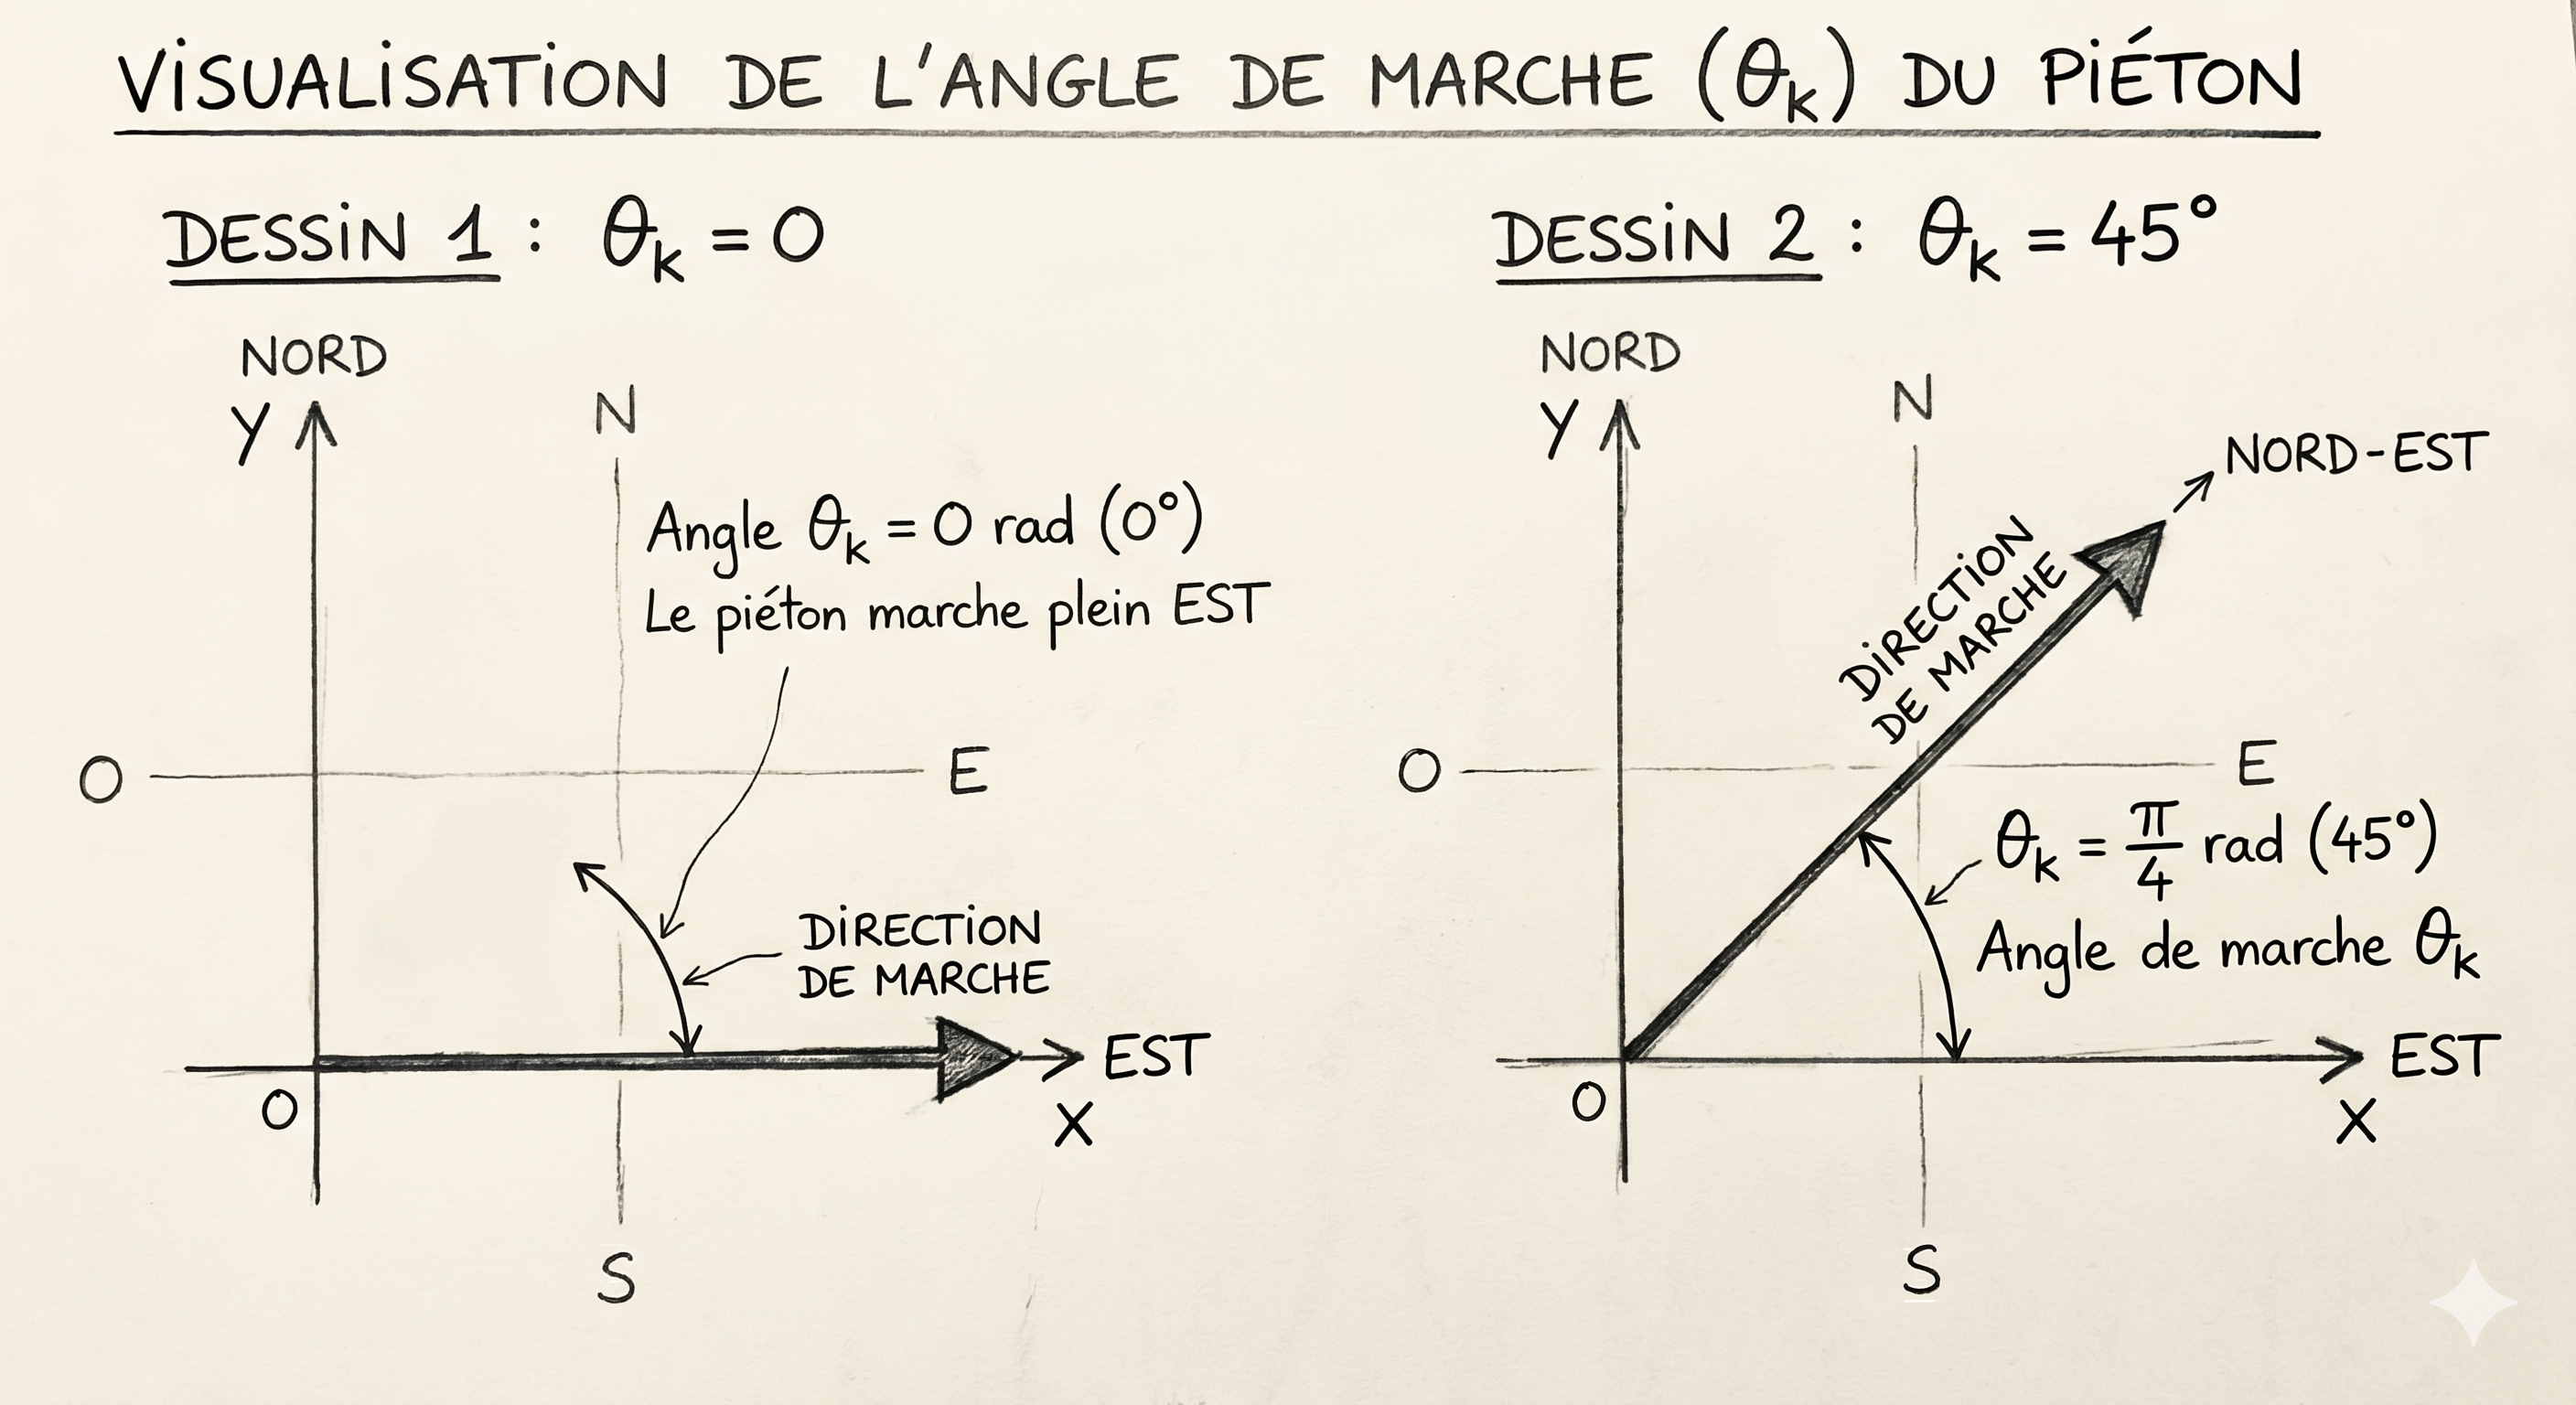
\includegraphics[width=0.5\textwidth]{images/model_boussole.png}
    \caption{Modèle de la boussole et repère Est-Nord}
    \label{fig:model_boussole}
\end{figure}

Le système est piloté par le vecteur de commande $U_k$ :
\begin{equation}
 U_k = \begin{bmatrix} v_k \\ \omega_k \end{bmatrix} 
\end{equation}
Où $v_k$ est la vitesse scalaire du piéton et $\omega_k$ la vitesse angulaire. 
Dans notre montage matériel, nous avons observé expérimentalement que l'accéléromètre mesurait systématiquement environ $1G$ (la gravité terrestre) sur l'axe X, tandis que les axes Y et Z restaient proches de $0G$. On en deduit que la carte Raspberry Pi était fixée de sorte que son axe X pointait verticalement vers le ciel. Donc la rotation du piéton sur lui-même correspond physiquement à une rotation autour de cet axe vertical, qui est lue directement par \textit{Gyro\_X} (IMU).

\begin{figure}[htbp]
    \centering
    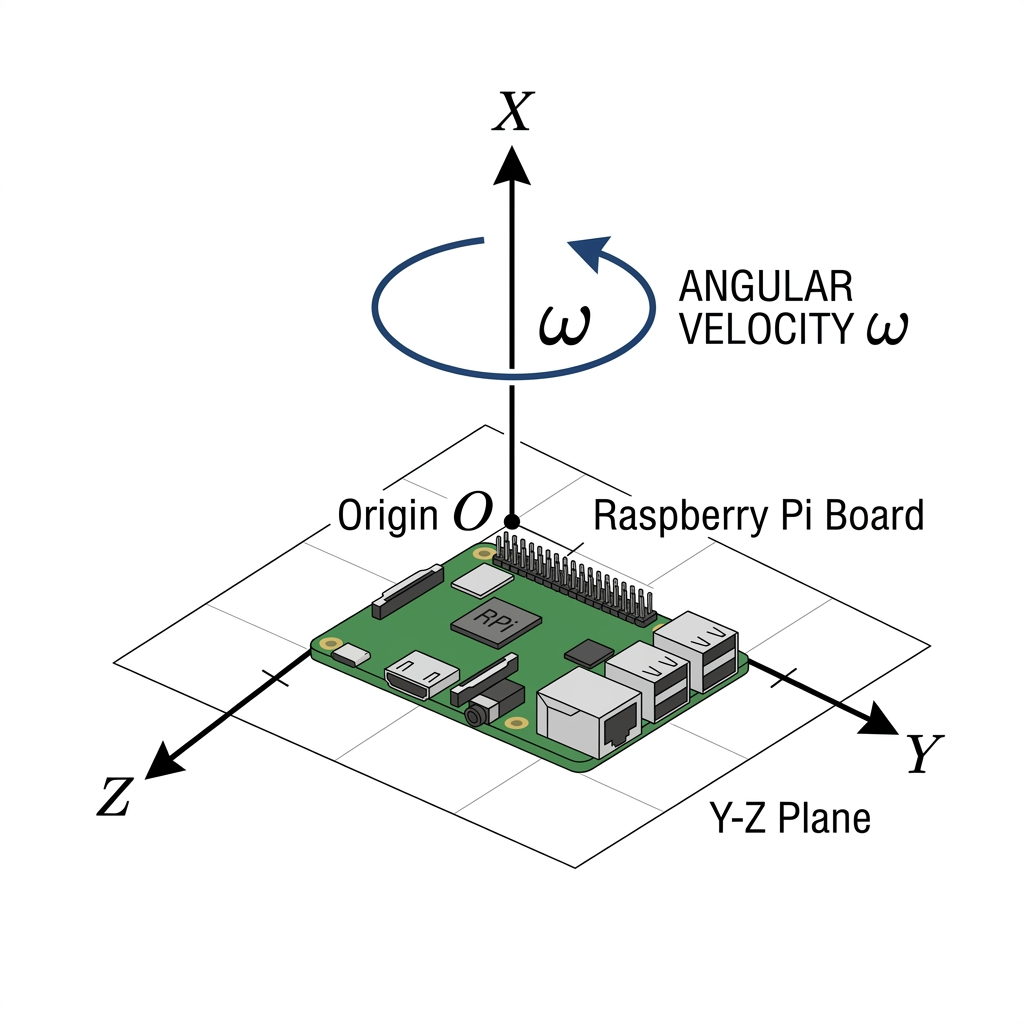
\includegraphics[width=0.5\textwidth]{images/diagramme_imu_axe_x.png}
    \caption{Montage matériel de l'IMU : l'axe X pointe vers le haut}
    \label{fig:diagramme_imu_axe_x}
\end{figure}

\subsubsection{Étape de Prédiction (Propagation)}
L'évolution de la position du piéton n'est pas linéaire à cause des fonctions trigonométriques. Le modèle non-linéaire $f$ se traduit par les équations de mécanique classique :
\begin{equation}
 \begin{bmatrix} x_k \\ y_k \\ \theta_k \end{bmatrix} = \begin{bmatrix} x_{k-1} + v_k \cdot \cos(\theta_{k-1}) \cdot \Delta t \\ y_{k-1} + v_k \cdot \sin(\theta_{k-1}) \cdot \Delta t \\ \theta_{k-1} + \omega_k \cdot \Delta t \end{bmatrix} 
\end{equation}

\begin{figure}[htbp]
    \centering
    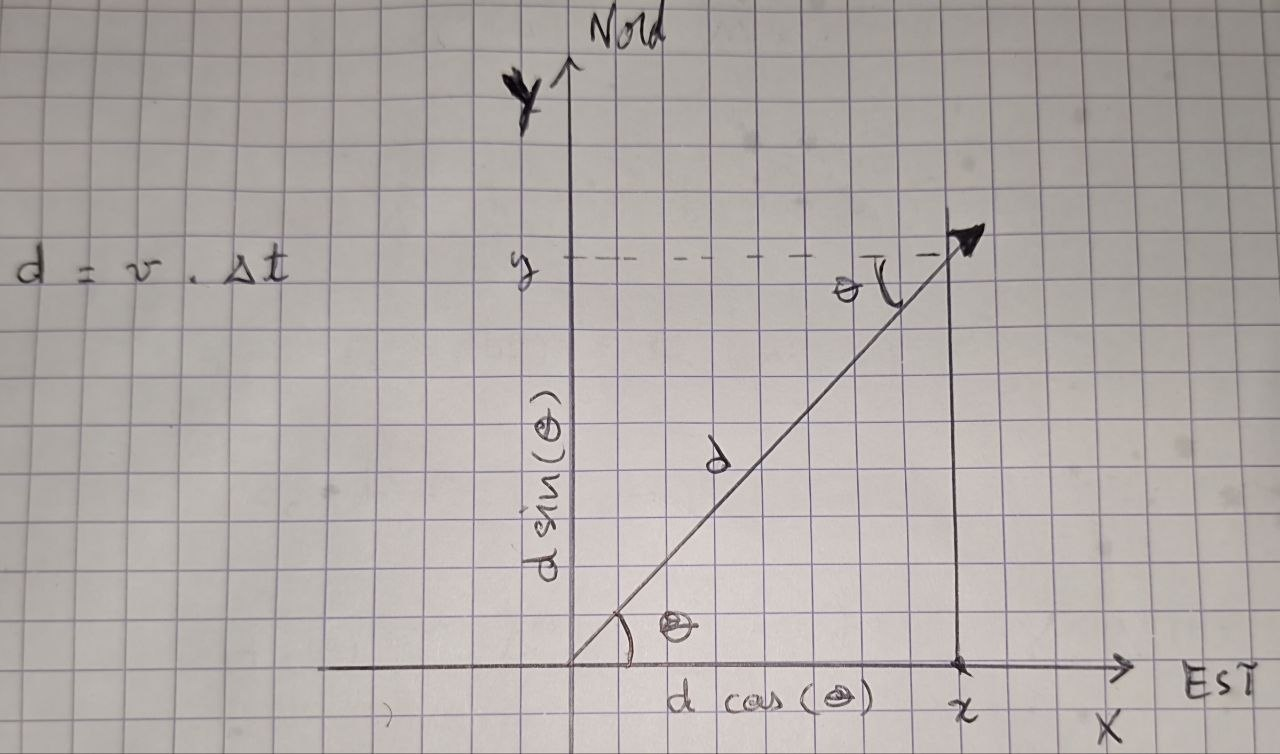
\includegraphics[width=0.5\textwidth]{images/trigo_cinematique.jpg}
    \caption{Projection trigonométrique du déplacement $v \cdot \Delta t$ sur les axes Est ($X$) et Nord ($Y$)}
    \label{fig:trigo_cinematique}
\end{figure}

Pour appliquer le filtre de Kalman, nous devons linéariser cette fonction en calculant sa Jacobienne $F_k$ :
\begin{equation}
 F_k = \frac{\partial f}{\partial X} = \begin{bmatrix} 1 & 0 & -v_k \cdot \sin(\theta_{k-1}) \cdot \Delta t \\ 0 & 1 & v_k \cdot \cos(\theta_{k-1}) \cdot \Delta t \\ 0 & 0 & 1 \end{bmatrix} 
\end{equation}

\textbf{Matrice de Bruit de Processus ($Q$)} \\
La matrice de covariance $Q$ représente l'incertitude de notre prédiction. Issue du modèle \textbf{CWNA} (\textit{Continuous White Noise Acceleration}, réf. CM6), elle se modélise par :
\begin{equation}
 Q = \begin{bmatrix} \frac{\sigma_a^2 \cdot \Delta t^4}{4} & 0 & 0 \\ 0 & \frac{\sigma_a^2 \cdot \Delta t^4}{4} & 0 \\ 0 & 0 & \sigma_\omega^2 \cdot \Delta t^2 \end{bmatrix} 
\end{equation}
Ici, $\sigma_a$ est recalculé dynamiquement à chaque itération via la variance de l'accélération horizontale de l'IMU, permettant au filtre de s'adapter à la force réelle du pas de l'utilisateur.
La prédiction de la covariance devient alors : $P_{k|k-1} = F_k P_{k-1|k-1} F_k^T + Q$.

\subsubsection{Étape de Correction (Mise à jour GPS)}
Nous mesurons uniquement la position $(x, y)$ grâce au GPS. La matrice d'observation $H$ est donc linéaire :
\begin{equation}
 H = \begin{bmatrix} 1 & 0 & 0 \\ 0 & 1 & 0 \end{bmatrix} 
\end{equation}

La matrice $R$ représente l'imprécision du GPS, obtenue expérimentalement lors de nos tests :
\begin{equation}
 R = \begin{bmatrix} 1.20 & 0 \\ 0 & 0.07 \end{bmatrix} 
\end{equation}

\textbf{Filtre Anti-Outliers (Distance de Mahalanobis)} \\
Afin de rejeter les mesures GPS aberrantes (phénomène de \textit{multipath} ou pertes de signal temporaires), nous avons implémenté une technique de \textit{gating} probabiliste basée sur la distance de Mahalanobis. Avant d'accepter une mesure GPS, nous calculons l'innovation $\tilde{y} = Z_k - H \hat{X}_{k|k-1}$ et sa covariance $S = H P_{k|k-1} H^T + R$.
Nous évaluons ensuite la distance de Mahalanobis au carré : $d^2 = \tilde{y}^T S^{-1} \tilde{y}$. 

Statistiquement, les résidus normalisés d'un filtre de Kalman optimal suivent une loi du $\chi^2$ (Khi-deux). Pour notre système d'observation 2D (X et Y), nous avons 2 degrés de liberté.
Pour rejeter les données aberrantes avec un intervalle de confiance de 99\%, le seuil théorique tabulé est de $9.21$ (\textit{Réf : Tables statistiques du $\chi^2$ / Théorie de l'estimation et du filtrage optimal}). 
Ainsi, si $d^2 > 9.21$, la mesure GPS est considérée comme une anomalie et est purement ignorée, laissant le modèle inertiel prendre le relais pour garantir la fluidité de la trajectoire.

Si la mesure est valide, nous calculons le gain de Kalman $K$ et corrigeons l'état :
\begin{align}
   K &= P_{k|k-1} H^T S^{-1} \\
   \hat{X}_{k|k} &= \hat{X}_{k|k-1} + K \tilde{y} \\
   P_{k|k} &= (I - K H) P_{k|k-1}
\end{align}

\subsection{Critique et Limites du Modèle}

Bien que robuste face aux interférences magnétiques et au bruit d'accélération, notre modèle EKF cinématique repose sur plusieurs hypothèses:

\begin{enumerate}
    \item \textbf{Dépendance à la vitesse déduite du GPS} : Actuellement, la vitesse scalaire $v_k$ est calculée à partir de la différence de position entre deux points GPS successifs. Une amélioration  consisterait à récupérer et utiliser directement la vitesse \textit{Doppler} native fournie par la puce GPS (via les trames NMEA originelles). Cette vitesse matérielle est nettement plus instantanée et fiable que la dérivation spatiale. De plus, si le signal GPS est totalement perdu (ex: tunnel prolongé), notre vitesse calculée tombe à zéro, empêchant toute vraie navigation (mais cela peut se resoudre en integrant temporairement l'acceleration).
    \item \textbf{Dérive résiduelle du Gyroscope (Drift)} : En l'absence d'un cap absolu (le magnétomètre ayant été écarté du modèle en raison des perturbations environnementales), l'intégration numérique de la vitesse angulaire $\omega_k$ finira inévitablement par dériver au bout de plusieurs dizaines de minutes de marche, malgré notre calibration statique du biais initial.
    \item \textbf{Hypothèse de mouvement rectiligne aligné} : Le modèle cinématique suppose que le piéton avance en permanence de manière parfaitement alignée avec l'axe de visée de la carte (cap $\theta$). Cette restriction rend le modèle incapable d'estimer correctement la trajectoire lors de mouvements tels que les pas chassés ou les marches en reculant ... (personne ne fait ça normalement)
\end{enumerate}

Nous avons pas pu exploiter le magnetomètre comme il se devait il resoudrait bon nombre de nos problèmes.

\subsection{Analyse des résultats}
L'évaluation des performances de l'EKF cinématique repose sur une comparaison
visuelle avec la vérité terrain Strava, acquise simultanément lors de trois
parcours distincts sur le campus de l'INSA Rouen. Chaque carte superpose
cinq couches : la vérité terrain Strava (noir), le GPS brut avant filtrage
(gris), le GPS nettoyé utilisé par le filtre (rouge), les points GPS rejetés
par le gate de Mahalanobis (orange), et la trajectoire estimée par l'EKF
(bleu).

\subsubsection{Terrain dégagé — grand parcours}

Sur un parcours de grande envergure en terrain dégagé
(Figure~\ref{fig:trajet_grand}), la trajectoire EKF (bleu) suit fidèlement
le GPS nettoyé (rouge) et reste à quelques mètres de la vérité terrain
Strava (noir). L'absence de points orange indique que le filtre de
Mahalanobis n'a rejeté aucune mesure GPS sur ce parcours : les conditions
extérieures dégagées produisent un signal GNSS de qualité, sans anomalie
détectable. La trajectoire EKF apparaît légèrement plus lisse que le GPS
nettoyé brut, ce qui confirme le rôle régularisateur du filtre.


\begin{figure}[H]
    \centering
    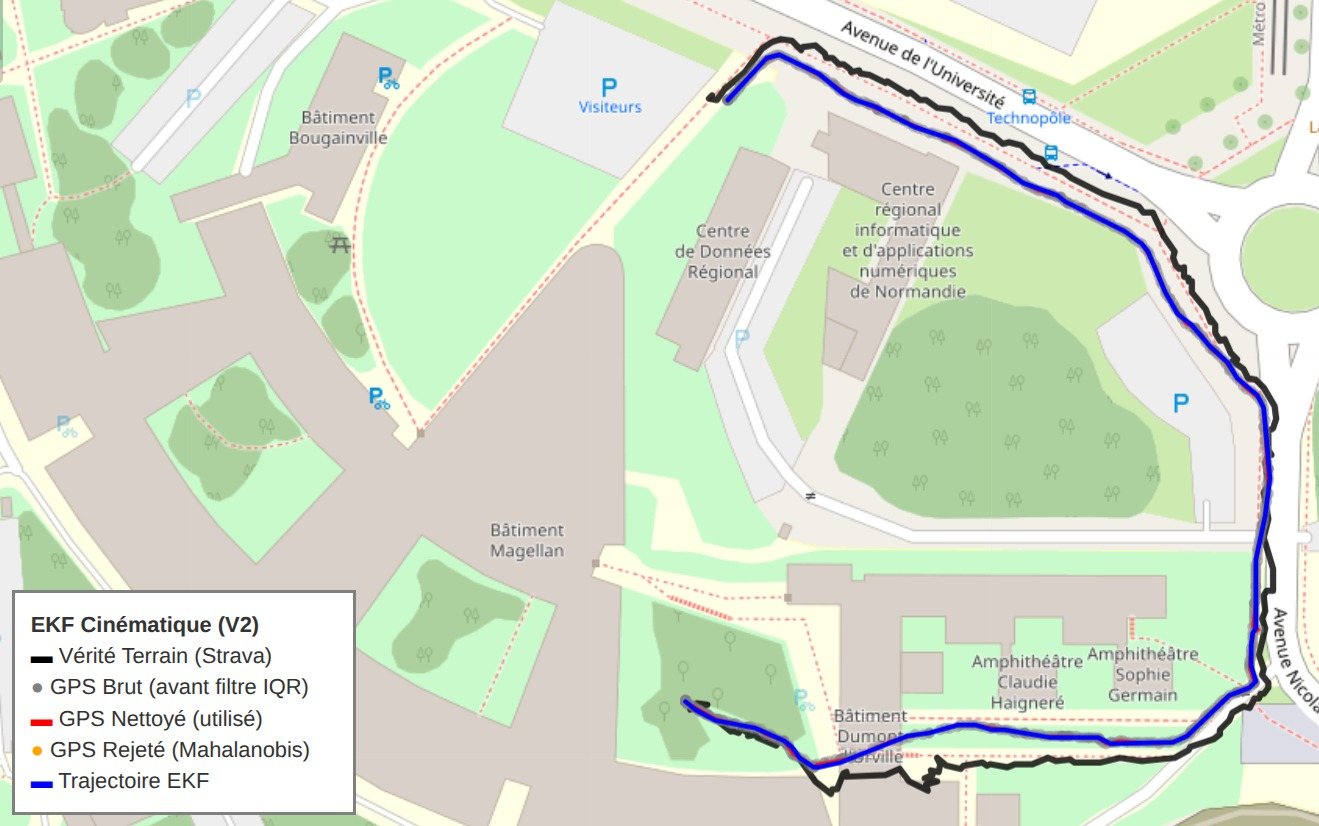
\includegraphics[width=0.65\textwidth]{images/trajet_plus_grand.jpeg}
    \caption{EKF cinématique sur grand parcours extérieur — campus INSA Rouen}
    \label{fig:trajet_grand}
\end{figure}



\subsubsection{Petit parcours — analyse des écarts}

Sur un trajet plus court (Figure~\ref{fig:trajet_petit}), un décalage
systématique apparaît entre notre estimation (rouge/bleu) et la vérité
terrain Strava (noir). Ce décalage, de l'ordre de quelques mètres, peut
s'expliquer par deux phénomènes distincts. D'une part, Strava utilise un
algorithme de \textit{map-matching} qui projette les positions GPS sur les
chemins connus de la carte, introduisant un biais artificiel par rapport
à la trajectoire réelle. D'autre part, l'imprécision résiduelle de notre
récepteur GNSS, modélisée par la matrice $R$, génère un décalage
incompressible même après filtrage. Ces deux sources d'erreur rendent
la comparaison absolue difficile, et justifient d'interpréter les résultats
de manière relative plutôt qu'absolue.


\begin{figure}[H]
    \centering
    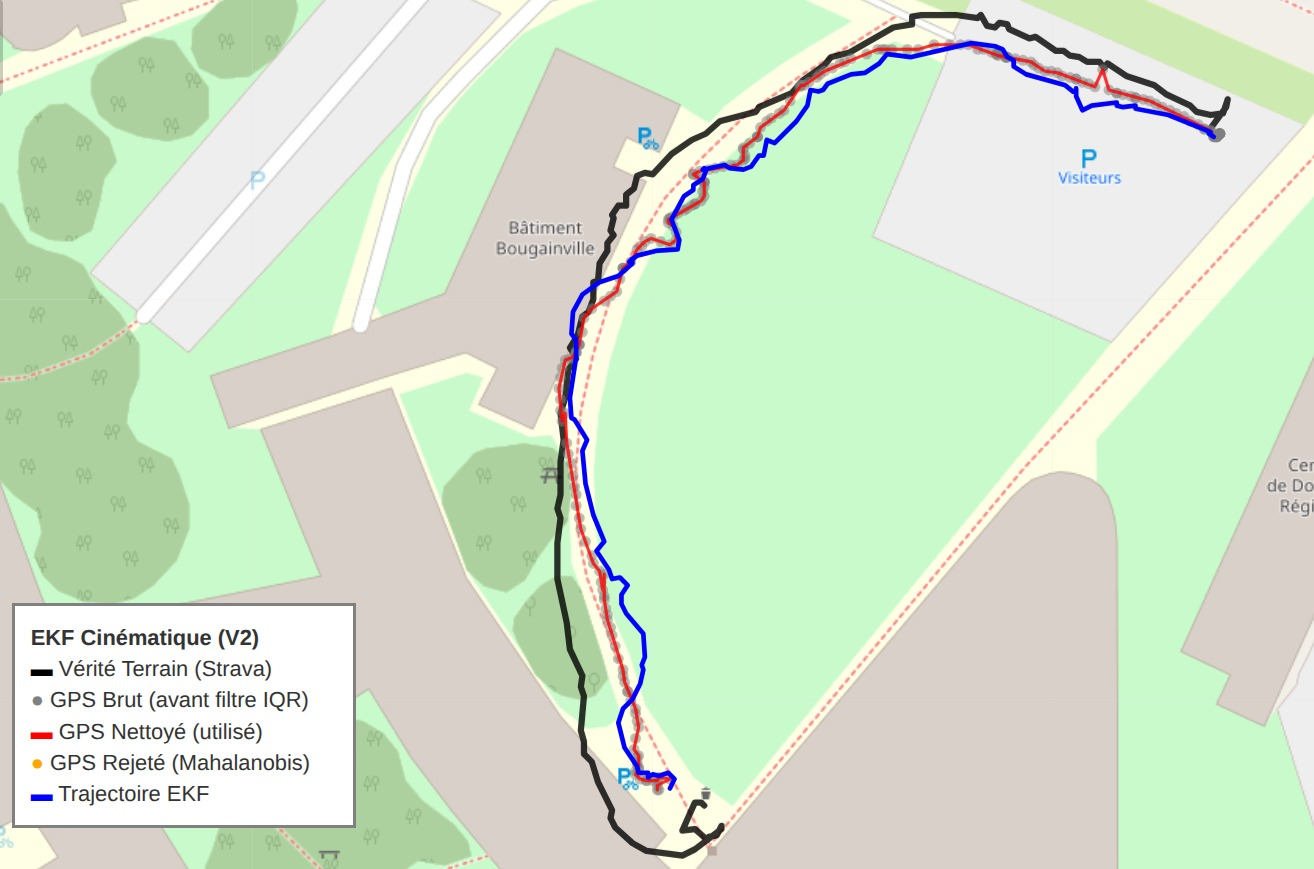
\includegraphics[width=0.65\textwidth]{images/trajet_petit.jpeg}
    \caption{EKF cinématique sur petit parcours — comparaison avec Strava}
    \label{fig:trajet_petit}
\end{figure}



\subsubsection{Passage en intérieur — robustesse du filtre}

Le troisième parcours (Figure~\ref{fig:trajet_ascenseur}) constitue le cas
le plus instructif. Lors d'un passage en intérieur (ascenseur et couloirs),
le signal GNSS subit de fortes perturbations de type \textit{multipath} :
les réflexions sur les murs produisent des positions aberrantes, visibles
sous forme d'un large nuage de points orange dans la partie inférieure de
la carte. Le gate de Mahalanobis a correctement identifié et rejeté
l'intégralité de ces mesures corrompues.

Durant cette phase de dégradation GPS, l'EKF a maintenu une trajectoire
continue et physiquement cohérente (bleu) en s'appuyant uniquement sur
le modèle cinématique. Ce comportement illustre concrètement l'apport de
la fusion multi-capteurs : là où un GPS seul produirait une trajectoire
erratique, le filtre de Kalman assure la continuité de l'estimation.

On notera que la vérité terrain Strava (noir) présente elle-même un
comportement erratique dans la même zone, confirmant que les perturbations
GNSS en intérieur affectent tous les récepteurs, y compris les smartphones
modernes.



\begin{figure}[H]
    \centering
    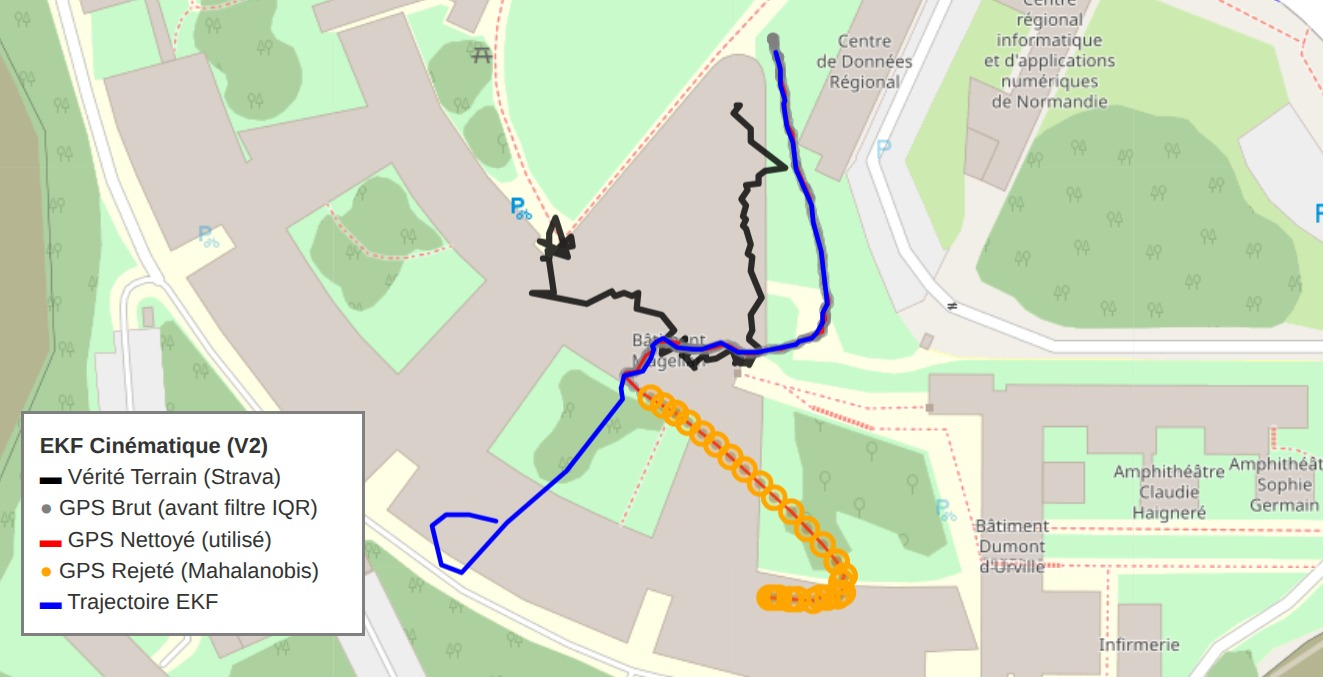
\includegraphics[width=0.65\textwidth]{images/trajet_avec_ascenceur.jpeg}
    \caption{Rejet Mahalanobis lors d'un passage en intérieur — EKF en navigation autonome}
    \label{fig:trajet_ascenseur}
\end{figure}



\subsubsection{Bilan}

Les trois acquisitions mettent en évidence les points suivants :

\begin{itemize}
    \item \textbf{En terrain dégagé}, l'EKF produit une trajectoire lisse
    et cohérente, très proche de la vérité terrain.
    \item \textbf{En conditions dégradées} (intérieur, multipath), le gate
    de Mahalanobis rejette efficacement les mesures corrompues et l'EKF
    maintient une estimation continue grâce au modèle cinématique.
    \item \textbf{Un décalage résiduel} de quelques mètres persiste entre
    notre estimation et Strava, attribuable en partie au map-matching de
    Strava et en partie à la précision intrinsèque du récepteur GNSS.
\end{itemize}

\section{Fonctionnalité supplémentaire}
\subsection{L'idée initiale}
Suite à une première concertation au sein du groupe, nous avons décidé de coder une fonctionnalité qui nous permettrait de localiser des photos prises sur une carte. Après consultation avec les professeurs, nous avons ajouter à cette idée une fonctionnalité de résolution de parcours. Cette dernière, nous permet de créer une sorte de GeoGuessr. 

La fonctionnalité se décompose en deux scripts distincts :
\textit{construire\_parcours.py} pour la création du parcours, et
\textit{resoudre\_parcours.py} pour la résolution.

\subsection{Capteurs sollicités}

Quatre capteurs sont mobilisés dans cette fonctionnalité :

\begin{itemize}
    \item \textbf{Module GNSS} : fournit la position absolue du joueur en
    latitude/longitude. Utilisé à la fois lors de la construction (enregistrement
    des coordonnées des checkpoints) et lors de la résolution (estimation de
    la proximité d'un checkpoint).
    \item \textbf{IMU} : complète le GPS en temps réel via le filtre de Kalman,
    assurant une estimation de position continue entre deux fixes GPS.
    \item \textbf{Caméra (RPi Camera Module 3)} : capture des photos de
    référence lors de la construction, et des photos de vérification lors de
    la résolution. Les images sont comparées par un algorithme de mise en
    correspondance de points caractéristiques.
    \item \textbf{Buzzer} : fournit un retour audio au joueur une mélodie
    courte pour un checkpoint validé, une mélodie plus longue pour la
    complétion du parcours.
\end{itemize}

Un écran LCD et un bouton poussoir complètent l'interface utilisateur.

\subsection{Architecture logicielle}

Le script de résolution repose sur une architecture multi-threadée à trois
fils d'exécution parallèles :

\begin{itemize}
    \item \textbf{Thread GPS} : appelle \texttt{gnss\_position()} en continu
    et envoie les trames de position dans une queue partagée.
    \item \textbf{Thread IMU} : appelle \texttt{get\_imu\_data()} en continu
    et envoie les données inertielles dans la même queue.
    \item \textbf{Thread fusion} : consomme la queue, alimente le filtre de
    Kalman et met à jour la position estimée \texttt{last\_kalman\_pos}.
\end{itemize}

Le thread principal effectue un polling du bouton poussoir et déclenche la
vérification de checkpoint sur appui.

\subsection{Implémentation}

\subsubsection{Construction du parcours}

Lors de la construction, l'opérateur se déplace de point en point sur le
campus. À chaque checkpoint, il peut prendre plusieurs photos de référence
via un \textbf{appui court} (moins de 1.5 secondes) sur le bouton, puis
valider le checkpoint par un \textbf{appui long} (plus de 1.5 secondes).
La possibilité de prendre plusieurs photos de référence par checkpoint
améliore la robustesse de la validation visuelle ultérieure.

Les données sont enregistrées dans un fichier \texttt{parcours.txt} au
format suivant :

\begin{verbatim}
img1.jpg,img2.jpg;49.3845;1.0686
img3.jpg;49.3850;1.0690
\end{verbatim}

Chaque ligne correspond à un checkpoint : la liste des images de référence
séparées par des virgules, suivie des coordonnées GPS latitude et longitude.

\subsubsection{Résolution du parcours}

Au lancement, le script génère automatiquement une carte Folium affichant
les checkpoints avec leurs photos de référence en popup, permettant au joueur
de visualiser les emplacements à atteindre.

La validation d'un checkpoint se déroule en deux étapes successives :

\begin{enumerate}
    \item \textbf{Validation géographique} : sur appui bouton, la distance
    entre la position Kalman estimée et le checkpoint est calculée via la
    formule géodésique. Si cette distance est inférieure à 25 mètres, la
    vérification visuelle est déclenchée.
    \item \textbf{Validation visuelle} : une photo est capturée et comparée
    aux images de référence du checkpoint par l'algorithme ORB. Si le score
    de correspondance dépasse le seuil, le checkpoint est validé.
\end{enumerate}

Ce double critère proximité GPS \textit{et} reconnaissance visuelle
réduit les faux positifs : être proche d'un checkpoint ne suffit pas,
il faut également photographier le bon élément visuel.

\begin{figure}[htbp]
    \centering
    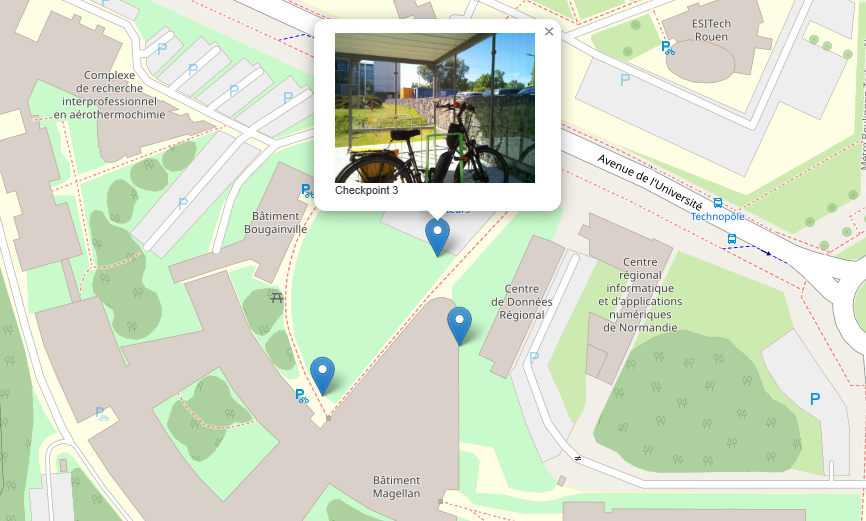
\includegraphics[width=0.85\textwidth]{images/carte_folium.png}
    \caption{Carte Folium générée au lancement de \texttt{resoudre\_parcours.py}
    les marqueurs indiquent les checkpoints du parcours. Au clic, une popup
    affiche la photo de référence à retrouver.}
    \label{fig:carte_folium}
\end{figure}

\subsubsection{Fusion GPS/IMU en temps réel}

La position du joueur est estimée en continu par un filtre de Kalman
fonctionnant selon le modèle à vitesse constante décrit en
section~\ref{sec:ekf}. Les paramètres sont identiques à ceux calibrés
pour la Partie 1 :

\begin{equation}
    R = \begin{bmatrix} 1.20 & 0 \\ 0 & 0.07 \end{bmatrix} \text{ m}^2,
    \qquad \sigma_a = 0.86 \text{ m/s}^2
\end{equation}

\subsubsection{Validation visuelle par ORB}

L'algorithme ORB (\textit{Oriented FAST and Rotated BRIEF}) est un
détecteur de points caractéristiques invariant aux rotations et aux
changements d'échelle. Pour chaque paire d'images, il extrait jusqu'à
2000 points d'intérêt et calcule leurs descripteurs binaires. La mise
en correspondance est effectuée par un \texttt{BFMatcher} à distance de
Hamming, avec filtre à distance inférieure à 50.

Lorsque plusieurs images de référence sont disponibles pour un checkpoint,
le meilleur score parmi toutes les comparaisons est retenu :

\begin{equation}
    \text{score} = \min\left(\frac{N_{\text{matches}}}{2000} \times 100,\ 100\right) \%
\end{equation}

Le checkpoint est validé si le nombre de correspondances dépasse
$N_{\text{min}} = 400$. Ce seuil a été fixé expérimentalement.


\subsubsection{Fonctionnement détaillé de l'algorithme ORB}

ORB (\textit{Oriented FAST and Rotated BRIEF}) est un algorithme de
détection et description de points caractéristiques, développé comme
alternative rapide à SIFT et SURF. Il se compose de deux étapes
successives.

\paragraph{Détection des points clés}
FAST (\textit{Features from Accelerated Segment Test}) identifie les
points d'intérêt dans une image en analysant l'intensité des pixels
sur un cercle de 16 pixels autour de chaque candidat. Un point est
retenu comme coin si un arc suffisamment long de pixels consécutifs
est significativement plus clair ou plus sombre que le pixel central.
ORB ajoute à FAST une composante d'orientation : un gradient d'intensité
local est calculé pour attribuer un angle à chaque point détecté, rendant
le descripteur invariant aux rotations.

\paragraph{Description}
BRIEF (\textit{Binary Robust Independent Elementary Features}) représente
chaque point clé par un vecteur binaire construit à partir de comparaisons
d'intensité entre paires de pixels dans un voisinage local. La version
\textit{Rotated} de ORB oriente ces comparaisons selon l'angle calculé
par FAST, garantissant ainsi l'invariance rotationnelle du descripteur.

\paragraph{Mise en correspondance}
Les descripteurs binaires sont comparés par distance de Hamming (nombre
de bits différents entre deux descripteurs). Un \texttt{BFMatcher}
(\textit{Brute-Force Matcher}) compare exhaustivement chaque descripteur
de l'image de test contre tous ceux de l'image de référence, et retient
les paires dont la distance est inférieure à 50.

\begin{figure}[htbp]
    \centering
    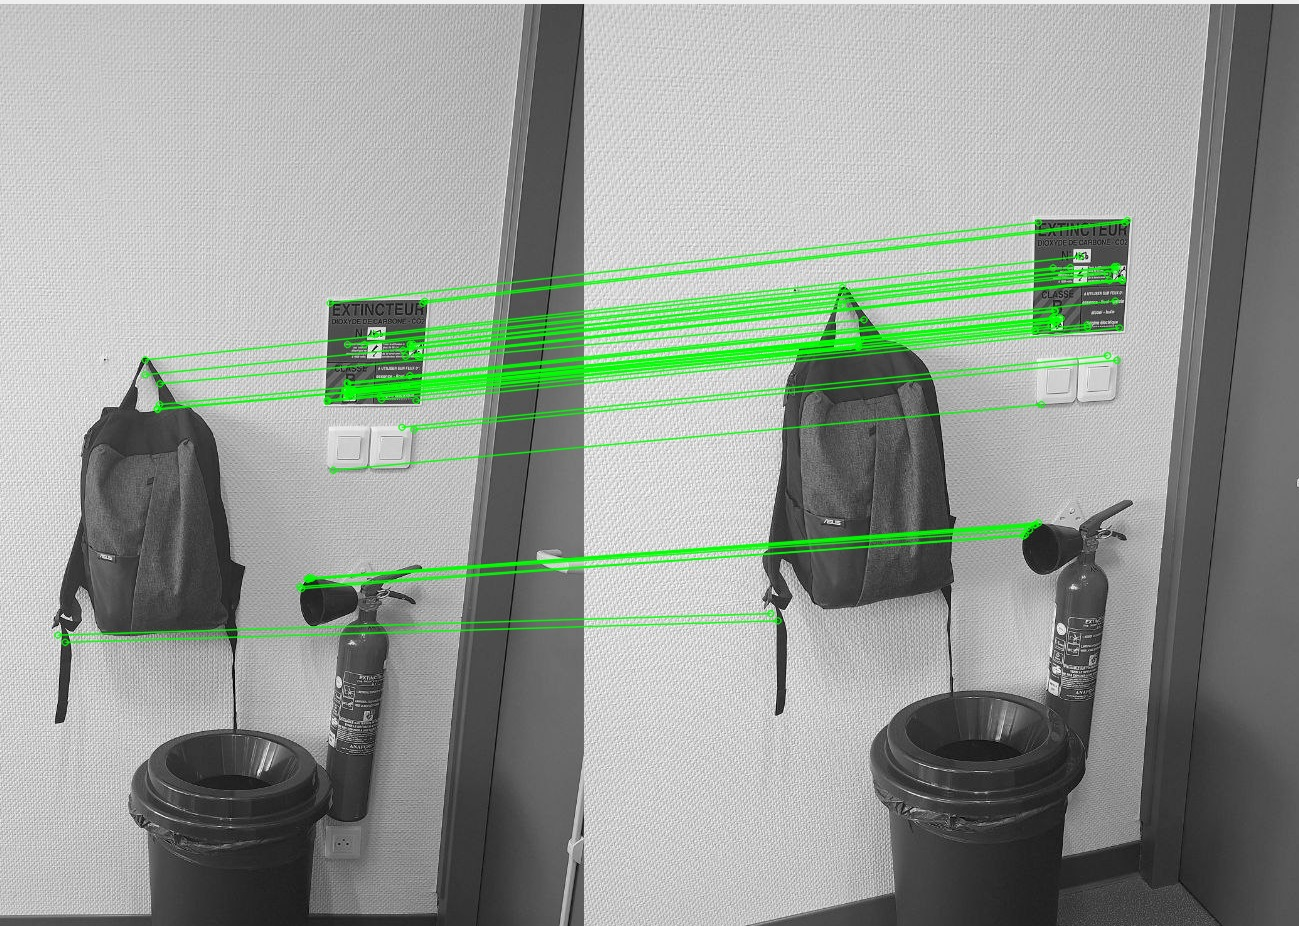
\includegraphics[width=0.95\textwidth]{images/orb_matching.jpeg}
    \caption{Visualisation des correspondances ORB entre deux photos du
    même checkpoint (image gauche : référence, image droite : vérification).
    Les lignes vertes relient les points caractéristiques mis en
    correspondance la densité et la cohérence géométrique des lignes
    indiquent une reconnaissance réussie.}
    \label{fig:orb_matching}
\end{figure}

La Figure~\ref{fig:orb_matching} illustre un cas de validation réussie :
les correspondances s'établissent sur des éléments texturés stables
(extincteur, panneau mural, interrupteurs), répartis sur l'ensemble
de l'image. Cette distribution spatiale large est caractéristique
d'une vraie reconnaissance et non d'une coïncidence locale.

\subsubsection{Retour utilisateur LCD et buzzer}

À chaque action du joueur, un retour immédiat est fourni via l'écran LCD
et le buzzer. Le tableau suivant récapitule les messages affichés selon
les situations :

\begin{table}[H]
    \centering
    \caption{Messages LCD selon l'état du système}
    \begin{tabular}{ll}
        \hline
        \textbf{Situation} & \textbf{Affichage LCD} \\
        \hline
        Démarrage           & \texttt{Appuyez bouton} \\
        Capture en cours    & \texttt{Photo en cours...} \\
        Trop loin           & \texttt{Trop loin...} \\
        Photo non reconnue  & \texttt{Mauvais endroit!} + score \% \\
        Checkpoint validé   & \texttt{CP X valide !} + score \% \\
        Parcours terminé    & \texttt{Bravo ! Fini !} \\
        \hline
    \end{tabular}
\end{table}

Le score affiché correspond au pourcentage de correspondances ORB
($N_{\text{matches}} / 2000 \times 100$), permettant au joueur de savoir
s'il était proche de valider ou complètement hors sujet.

Le buzzer fournit un retour audio complémentaire : une mélodie courte signale la validation d'un checkpoint, tandis qu'une mélodie
plus longue célèbre la complétion du parcours entier. Ces signaux permettent
au joueur de jouer sans regarder l'écran en permanence.



\subsection{Outils et bibliothèques utilisés}

La fonctionnalité mobilise plusieurs outils et bibliothèques vus en ITI3 :

\begin{itemize}
    \item \textbf{threading / queue} : architecture multi-threadée pour
    l'acquisition simultanée GPS et IMU, avec synchronisation par file
    d'attente partagée paradigme de programmation concurrente vu en
    cours système.
    \item \textbf{GPIO / PWM} : contrôle du buzzer par modulation de
    largeur d'impulsion et polling du bouton poussoir, utilisés en TP
    Capteurs.
    \item \textbf{Folium} : génération de la carte interactive OpenStreetMap
    avec les checkpoints en popup.
    \item \textbf{RPLCD} : affichage du score de correspondance et des
    messages de validation sur l'écran LCD I2C en temps réel.
    \item \textbf{subprocess / rpicam-still} : déclenchement de la caméra
    RPi Camera Module 3 depuis Python pour la capture des photos.
\end{itemize}

\subsection{Analyse critique}

La fonctionnalité a été testée sur le campus avec des parcours de 3 à 5
checkpoints. Les résultats sont globalement satisfaisants : les checkpoints
étaient retrouvés et validés correctement, avec une fiabilité variable selon
les conditions.

Plusieurs limitations ont été identifiées :

\begin{enumerate}
    \item \textbf{Dépendance à la vitesse de marche} : le modèle cinématique
    à vitesse constante du filtre de Kalman suppose un déplacement régulier.
    Une marche rapide dégrade la précision de l'estimation de position entre
    deux fixes GPS, ce qui peut empêcher la détection de proximité à 25 mètres.
    En pratique, un rythme de marche modéré était nécessaire pour un
    fonctionnement fiable.

    \item \textbf{Sensibilité aux conditions d'éclairage} : l'algorithme ORB
    est sensible aux variations d'éclairage entre la phase de construction et
    la phase de résolution. Un changement de luminosité important (ciel couvert
    vs ensoleillé) réduit le nombre de correspondances et peut provoquer des
    faux négatifs.

    \item \textbf{Seuil ORB empirique} : le seuil de 400 correspondances a
    été fixé par expérimentation. Il ne repose pas sur un modèle statistique
    formel, ce qui le rend potentiellement fragile face à des scènes peu
    texturées ou à des angles de prise de vue trop différents entre la
    référence et la vérification.

    \item \textbf{Seuil GPS de 25 mètres} : ce seuil est volontairement large
    pour compenser les imprécisions du GPS en extérieur. Sans la validation
    visuelle ORB, il serait insuffisant pour discriminer des checkpoints
    proches les uns des autres.
\end{enumerate}



L'utilisation conjointe de la proximité GPS et de la reconnaissance visuelle
constitue un choix de conception robuste : les deux modalités se compensent
mutuellement. Une piste d'amélioration serait de remplacer ORB par un
réseau de neurones convolutif pré-entraîné, plus robuste aux variations
d'éclairage et de point de vue.

\section{Difficultés rencontrées}
L'obtention d'une version stable à rencontrer de nombreux obstacles, tant sur le plan algorithmique que matériel, nécessitant le développement de plusieurs versions successives du filtre de Kalman avant d'aboutir à un résultat concluant. Cette section détaille les défis majeurs rencontrés par l'équipe et les solutions techniques apportées.

\subsection{Instabilités et refontes du filtre de kalman étendu (EKF)}
Le développement de l'algorithme de fusion a exigé une étroite adaptation face à la nature et aux imperfections des bruits des capteurs physiques :

\begin{itemize}
    \item \textbf{Interférences magnétiques majeures :} Initialement, le magnétomètre devait fournir un cap absolu pour orienter le système. Cependant, l'environnement urbain environnant ainsi que les perturbations électromagnétiques internes générées par la carte elle-même rendaient les mesures aberrantes et inutilisables.
    \item \textit{Solution :} Pas de solution fiable n'ayant été trouvé l'équipe a opté pour l'abandon total du magnétomètre. L'architecture de l'EKF a été basculée sur un modèle purement cinématique où le cap $\theta_k$ est estimé par l'intégration temporelle de la vitesse angulaire $\omega$ fournie par le gyroscope.
    
    \item \textbf{Dérive exponentielle de l'accéléromètre :} Les premières versions du filtre s'appuyaient sur une double intégration numérique de l'accélération linéaire pour estimer la position. En pratique, le bruit haute fréquence du capteur combiné aux résidus de la gravité terrestre provoquait une dérive en $t^2$, rendant la trajectoire totalement aberrante en quelques secondes.
    \item \textit{Solution :} Arrêt définitif de l'intégration spatiale. L'accéléromètre a été relégué à un rôle purement statistique : il sert désormais uniquement à calculer l'énergie instantanée de la marche (via la méthode RMS) afin d'adapter dynamiquement la matrice de bruit de processus $Q$.
    
    \item \textbf{Absence de vitesse native GPS :} Le script d'acquisition final ne permettait pas de récupérer la vitesse Doppler directement issue de la puce GNSS, qui constitue pourtant la mesure de vitesse matérielle la plus instantanée et fiable.
    \item \textit{Solution :} La vitesse scalaire $v$ a dû être reconstruite artificiellement par dérivation spatiale (calcul de la distance géodésique entre deux trames GPS successives divisée par le pas de temps $\Delta t$) lors de l'étape de post-traitement.
    
    \item \textbf{Sauts de position GPS (Effet Multipath) :} En milieu urbain dense ou à proximité des bâtiments du campus, les réflexions des signaux satellitaires altéraient brutalement les mesures de position, ce qui dégradait fortement la trajectoire calculée par l'EKF.
    \item \textit{Solution :} Mise en place d'un filtre anti-outliers robuste (\textit{Validation Gate}) basé sur la distance de Mahalanobis. Ce système rejette statistiquement toute donnée dont le résidu normalisé est supérieur au seuil théorique du $\chi^2$ (fixé à $9.21$ pour 2 degrés de liberté), laissant le modèle inertiel autonome prendre temporairement le relais.
\end{itemize}

\subsection{Problématiques matérielles et intégration mécanique}
L'assemblage physique de l'ITIPhone sur sa plaquette d'essais a également ralenti la phase de prototypage en conditions réelles :

\begin{itemize}
    \item \textbf{Connexion du cable de la caméra :} Lors du montage initial, le câble plat de la camera a été branché à l'envers. Le diagnostic et la correction de cette erreur ont requis un temps important en raison de l'accès restreint imposé par le shield matériel fixé sur la carte Raspberry Pi.
    \item \textbf{Orientation physique du capteur optique :} La caméra a également été montée à l'envers sur son support, ce qui inversait la totalité des captures d'écran nécessaires au fonctionnement du GeoGuessr. Bien qu'une solution interne purement logicielle eût été réalisable en Python (via un retournement de matrice avec OpenCV), on a privilégié une correction mécanique en démontant et retournant le module pour garantir une cohérence matérielle propre.
\end{itemize}

\subsection{Calibration et qualité des premières acquisitions}
Lors des premières acquisitions en extérieur, les trajectoires brutes enregistrées par le module GPS seul présentaient un décalage très marqué et une forte imprécision par rapport au trajet réel. 

Le problème suivant a été identifié: la vitesse de marche influençait directement la qualité de la géométrie des signaux reçus. La solution retenue a consisté à réduire volontairement la vitesse de marche lors des acquisitions suivantes. Ce rythme plus modéré et régulier a permis de stabiliser le récepteur GNSS, afin d'obtenir des trajets beaucoup plus précis.

\subsection{Échec de l'implémentation du filtre de kalman simple en temps réel}
Une part importante du travail d'ingénierie a initialement été consacrée à la tentative d'exécuter un Filtre de Kalman simple (linéaire) en direct, c'est-à-dire en flux tendu au cours de l'acquisition des données embarquées. L'objectif était de pouvoir estimer et afficher une trajectoire corrigée de manière instantanée.

Cependant, les résultats expérimentaux obtenus n'ont pas été à la hauteur des attentes. Lors des essais en direct, la trajectoire estimée présentait des anomalies majeures sous forme de « pics » de position brutaux et erratiques, totalement absents du trajet initial et physiquement impossibles pour un déplacement piéton. Ces divergences et cette instabilité s'expliquaient par plusieurs facteurs critiques :

\begin{itemize}
    \item \textbf{Hypothèse de linéarité mise en défaut :} Le filtre de Kalman simple repose sur des équations de transition strictement linéaires. En direct, les approximations nécessaires pour maintenir ce cadre linéaire (notamment l'évolution des composantes de cap et de vitesse) se sont révélées insuffisantes face aux dynamiques réelles du porteur.
    \item \textbf{Désalignement temporel et latence :} Le flux direct imposait de gérer le désalignement temporel (\textit{jitter}) et l'asynchronisme entre les trames à haute fréquence de l'IMU (100 Hz) et celles du GPS (1 Hz). Les fluctuations du pas de temps $\Delta t$ injectaient des erreurs numériques critiques dans les matrices de prédiction.
\end{itemize}

Face à l'impossibilité d'obtenir une version finale stable d'un filtre de Kalman simple en temps réel, et au vu du temps de calcul requis pour tenter de traiter ces donées à la volée, on a pris la décision d'abandonner cette approche. Nous nous sommes ainsi réorientés vers une architecture de post-traitement des données, garantissant une convergence mathématique robuste et une trajectoire finale d'une bien meilleure fidélité.

\section{Voies d'amélioration}
Bien que le système que nous avons développé réponde aux exigences initiales de robustesse et de continuité de positionnement, plusieurs axes d'amélioration pourraient permettre d'en optimiser les performances et d'étendre ses capacités opérationnelles.

\subsection{Exploitation de la vitesse Doppler du GNSS}

Afin de limiter les effets du bruit de mesure induit par la dérivation spatiale des positions successives, une piste d'amélioration significative consisterait à exploiter directement les mesures de vitesse Doppler fournies par le récepteur GNSS. L'intégration de ces informations de vitesse au sein de la matrice d'observation de l'EKF permettrait d'améliorer la robustesse et la stabilité de l'estimation de la vitesse du porteur, en particulier lors des phases transitoires où les variations dynamiques sont les plus marquées.

\subsection{Calibration dynamique et gestion du magnétomètre}

L'abandon du magnétomètre a permis d'éviter les perturbations électromagnétiques locales, mais au prix d'une dérive à long terme du cap (yaw) calculé par l'IMU. L'implémentation d'un algorithme de calibration dynamique permettrait de réintégrer le magnétomètre et d'éviter les problèmes liés au cap.

\subsection{Optimisation et EKF en temps réel}

Des optimisations de l'EKF en temps réel tels que la gestion de la latence, l'asynchronisme et où l'implementation de bruits adaptatifs auraient permis de s'affranchir des compromis de réglages fixes. cela aurait pu offrir au système une résilience et une précision optimales face aux perturbations environnementales et aux contraintes computationnelles de la plateforme embarquée.

\subsection{Mode plus intéractif}

L'aspect ludique du GeoGuessr pourrait être enrichi par le calcul en temps réel d'un score de précision plus exacte grâce aux améliorations liées à la partie 1. De plus, l'interface utilisateur pourrait guider le joueur à l'aide d'indicateurs de direction (ex: boussole visuelle ou signaux sonores...) générés directement à partir des écarts de coordonnées calculés par le système.

\section{Réalisation du projet}
\subsection{Tableau de répartition du travail}

Le tableau suivant présente la répartition des tâches et l'implication de chaque membre de l'équipe dans les différentes parties du projet ITInéraire.

\begin{table}[H]
    \centering
    \renewcommand{\arraystretch}{1.3}
    \footnotesize % Réduit la police au lieu de forcer une "boîte" graphique
    \begin{tabular}{|l|c|c|c|c|c|}
        \hline
        \textbf{Composants du Projet} & \textbf{I. El Assad} & \textbf{M. Kamara} & \textbf{M. Ravier} & \textbf{J. Semy} & \textbf{I. Thomas} \\ \hline
        \textbf{Choix Techniques (capteurs, algos, ...)} & X & X & X & X & X \\ \hline
        \textbf{Assemblage Physique du ITIphone} &  &  &  & X & X \\ \hline
        \textbf{Développement de Kalman de base} & X & X & X &  &  \\ \hline
        \textbf{Développement de EKF} & X & X &  &  &  \\ \hline
        \textbf{Acquisitions Partie 1} &  & &  & X & X \\ \hline
        \textbf{Partie Construction du Geoguessr} & X & X & X &  &  \\ \hline
        \textbf{Partie Résolution du Geoguessr} & X & X &  &  &  \\ \hline
        \textbf{Acquisitions Partie 2} & X & X & X & X & X \\ \hline
        \textbf{Rédaction du Rapport} & X & X & X & X & X \\ \hline
        \textbf{Débogage Divers \& Validation Système} & X & X & X & X & X \\ \hline
        \textbf{Partage des Acquisitions}  &  &  &  & X &   \\ \hline
        \textbf{Gestion du GitLab} &  &  & X & X &  \\ \hline
    \end{tabular}
    \caption{Répartition des tâches au sein de l'équipe}
    \label{tab:repartition}
\end{table}

\subsection{Note sur l'usage de l'IA}

Dans le cadre du développement de ce projet, nous avons fait le choix d'utiliser des LLM comme outils de support technique. Leur usage s'est restreint à des tâches d'assistance au débogage, à l'optimisation de la structure du code et à la rédaction de certaines sections du rapport en s'appuyant sur nos idées. L'intégralité de la conception algorithmique, du paramétrage des filtres mathématiques, de la réalisation des acquisitions et de l'analyse critique des résultats demeure le fruit exclusif de la réflexion et du travail de l'équipe.


\section{Conclusion}
Le projet ITInéraire a permis de concevoir et d'implémenter un système de localisation embarqué robuste, capable de compenser les faiblesses d'un positionnement GNSS standard. En fusionnant les données satellites avec celles de l'IMU, nous avons pu générer une estimation de trajectoire continue et physiquement cohérente. 

Ce projet a été particulièrement intéressant d’un point de vue conception et intégration matérielle. Se rendre compte du fonctionnement réel et des limites des capteurs physiques (dérive de l'IMU, sauts du GNSS) est la clé pour comprendre comment développer et paramétrer un algorithme de fusion de données robuste comme le Filtre de Kalman Étendu.

De plus, ce projet a été l’occasion de confronter nos différents points de vue sur certains aspects conceptuels et mathématiques, notamment lors de l'abandon du magnétomètre ou du réglage des matrices de covariance. Mettre en lumière nos différentes façons de penser, se projeter sur les fonctionnalités interactives à implémenter pour la résolution du GeoGuessr, et la communication au sein du groupe ont permis de surmonter les obstacles techniques et de concevoir ce projet de manière réfléchie et réussie.

\end{document}